% main.tex -- TEACHING EXAMPLE generated from templates/paper (LNCS skeleton, skills/paper-playbook).
% Every measurement-like number is in ../EVIDENCE.md; audit: crbench audit-tex (see audit-tex.log).
% Build: make           (runs fetch_llncs.sh if llncs.cls is missing, then latexmk)
% Drivers: main.tex (anonymous submission), main_camera.tex (proceedings,
% de-anonymised), main_full.tex (full version for ePrint). One shared source.
\documentclass[runningheads]{llncs}   % add 'a4paper' if the CFP requires A4

\newif\iffull   \fullfalse   % proceedings/submission build vs full version
\newif\ifanon   \anontrue    % anonymous submission build
\ifdefined\buildfull   \fulltrue\anonfalse \fi   % set by main_full.tex
\ifdefined\buildcamera \anonfalse \fi            % set by main_camera.tex

\usepackage[T1]{fontenc}
\usepackage{lmodern}
\usepackage{amsmath,amssymb}
\usepackage{graphicx}
\usepackage{booktabs,multirow}
\usepackage[table]{xcolor}
\usepackage{algorithm}
\usepackage{algpseudocode}
\usepackage{tikz}
\usepackage[hidelinks]{hyperref}
\usepackage[capitalise,noabbrev]{cleveref}
% Do NOT load geometry or change fonts/spacing: desk-reject risk.

% macros.tex -- notation conventions (keep in sync with paper/NOTATION.md).
% Rule: one concept, one macro. Change the macro, never the call sites.

% ---- number sets and rings
\newcommand{\NN}{\mathbb{N}}
\newcommand{\ZZ}{\mathbb{Z}}
\newcommand{\QQ}{\mathbb{Q}}
\newcommand{\RR}{\mathbb{R}}
\newcommand{\FF}{\mathbb{F}}
\newcommand{\Fp}{\mathbb{F}_p}
\newcommand{\Zq}{\mathbb{Z}_q}
\newcommand{\Rq}{\mathcal{R}_q}                 % R_q = Z_q[X]/(Phi_m(X))
\newcommand{\Torus}{\mathbb{T}}

% ---- vectors, matrices, distributions
\newcommand{\vc}[1]{\mathbf{#1}}                  % vectors bold lower-case
\newcommand{\mat}[1]{\mathbf{#1}}                 % matrices bold upper-case
\newcommand{\sample}{\xleftarrow{\$}}
\newcommand{\Dist}{\mathcal{D}}
\newcommand{\negl}{\mathsf{negl}}
\newcommand{\secpar}{\lambda}

% ---- algorithms and schemes (sans-serif names)
\newcommand{\alg}[1]{\mathsf{#1}}
\newcommand{\KeyGen}{\alg{KeyGen}}
\newcommand{\Enc}{\alg{Enc}}
\newcommand{\Dec}{\alg{Dec}}
\newcommand{\Eval}{\alg{Eval}}
\newcommand{\ct}{\mathsf{ct}}
\newcommand{\pk}{\mathsf{pk}}
\newcommand{\sk}{\mathsf{sk}}

% ---- complexity and cost (one paper-wide cost currency)
\newcommand{\cost}{\operatorname{cost}}
\newcommand{\bigO}{O}
\DeclareMathOperator{\poly}{poly}

% ---- scheme / library names (text)
\newcommand{\TFHE}{\textsf{TFHE}}
\newcommand{\BGV}{\textsf{BGV}}
\newcommand{\CKKS}{\textsf{CKKS}}
\newcommand{\PSI}{\textsf{PSI}}

% ---- evidence tag (renders nothing; used by cross-check scripts)
\newcommand{\ev}[1]{}                            % usage: 3.4$\times$\ev{E12}

% ---- drafting helpers (remove before submission; grep for TODO)
\newcommand{\todo}[1]{\textcolor{red}{[TODO: #1]}}

\newcommand{\evid}[1]{}   % evidence tag checked by crbench audit-tex (renders nothing)
\newcommand{\MVPBS}{\textsf{MV-PBS}}
\newcommand{\PBSop}{\textsf{PBS}}

% Anonymity: empty PDF metadata and no embedded figure source paths.
\hypersetup{pdfauthor={},pdftitle={},pdfsubject={},pdfkeywords={}}
\ifdefined\pdfsuppressptexinfo \pdfsuppressptexinfo=-1 \fi

% Optional modest float/display glue tuning (proceedings build only), see
% skills/paper-playbook/sections/00_overall_structure.md.
\iffull\else
  \setlength{\textfloatsep}{10pt plus 2pt minus 2pt}
  \setlength{\intextsep}{8pt plus 2pt minus 2pt}
\fi

\begin{document}

\title{One Blind Rotation, Four Output Bits:\\ a Toy Study of Multi-Value Bootstrapping\\ for 4-bit S-boxes in TFHE\\ \normalsize(teaching example --- not a research result)}
\titlerunning{Toy study: multi-value PBS for 4-bit S-boxes}
\ifanon
  \author{Anonymous Submission}
  \institute{}
\else
  % authors.tex -- de-anonymised author block (camera-ready / full version only).
% TEACHING EXAMPLE: no real authors.
\author{crypto-research-agents case study}
\authorrunning{Case study}
\institute{Teaching example}
   % author block kept out of the anonymous source tree
\fi
\maketitle

% abstract.tex -- three-part paradigm (skills/paper-playbook/sections/02_abstract.md).
% TEACHING EXAMPLE. Every number carries an evidence tag and is in ../EVIDENCE.md.
\begin{abstract}
Programmable bootstrapping (PBS) evaluates any look-up table on a TFHE ciphertext, but one PBS
returns one output; a 4-bit S-box whose output bits are consumed separately therefore costs
four blind rotations~\cite{CJP21}. Multi-value bootstrapping~\cite{CIM19} (CT-RSA'19)
shares one blind rotation among several tables of the same input.

We re-derive the factorisation $T_f = v_0\cdot d_f$ for the standard one-padding-bit encoding,
show that $d_f$ has at most $p$ non-zero integer coefficients with $\|d_f\|^2\le p+2$, and give
the resulting output variance $\|d_f\|^2\sigma^2_{\mathrm{BR}}+\sigma^2_{\mathrm{KS}}$.

In a pure-Python toy TFHE (insecure parameters, single thread, CPU time), the PRESENT S-box
costs 75.4~ms\evid{E2} instead of 291.2~ms\evid{E1}, a 3.86× [3.79, 3.95]\evid{E3} speed-up,
which saturates for many tables (43.67×\evid{E9} for 64 tables). The price is noise: at a
deliberately noisy parameter set the S-box failure rate rises from 0/128 to 32/128.
All code, logs and falsification scripts are part of the case study.
\end{abstract}


% intro.tex -- funnel -> bottleneck -> open question -> contributions (TEACHING EXAMPLE).
\section{Introduction}\label{sec:intro}
TFHE~\cite{CGGI16,CGGI20} refreshes a ciphertext with a \emph{blind rotation} of a test
polynomial, a technique going back to FHEW~\cite{DM15}. Choosing the test polynomial evaluates
an arbitrary function during the refresh (programmable bootstrapping, \PBSop)~\cite{CJP21}.
The blind rotation dominates the cost, and it does not depend on the function: evaluating
$k$ functions of the \emph{same} input with $k$ independent \PBSop{} repeats it $k$ times.

A 4-bit S-box is the textbook instance. If the next layer is bit-sliced, the four output bits
are needed as four ciphertexts, i.e.\ four \PBSop{}. (If a single ciphertext of the nibble
suffices, one \PBSop{} with $f=S$ does the job and there is nothing to optimise.)
Carpov, Izabach\`ene and Mollimard~\cite{CIM19} observed that the test polynomials of many
functions share a common factor $v_0$, so one blind rotation of $v_0$ can serve all of them
(multi-value PBS, \MVPBS). Tree-based and multi-value variants for larger tables were studied
in~\cite{GBA21}; CMux-tree evaluation from GGSW inputs goes back to~\cite{CGGI17}.

\subsection{Contributions (of this toy study)}
\begin{itemize}
\item A self-contained derivation of the factorisation for the one-padding-bit encoding
  (\Cref{lem:factor}), the exact bound $\|d_f\|^2\le p+2$ for Boolean tables
  (\Cref{lem:norm}), and the output-variance formula (\Cref{thm:noise}).
\item A falsification-first evaluation: 3.86×\evid{E3} for the PRESENT S-box, sub-linear
  scaling in the number of tables, and a parameter set where the noise price becomes visible.
\end{itemize}
We make no novelty claim: everything here is known since~\cite{CIM19}.
          % 1 Intro, 1.1 Related Work, 1.2 Contributions, 1.3 Overview
% prelim.tex -- notation (TEACHING EXAMPLE).
\section{Preliminaries}\label{sec:prelim}
Let $q=2^{32}$, $R=\ZZ[X]/(X^N+1)$ with $N$ a power of two, and $\Rq=R/qR$. Messages % no-evidence: q is a parameter definition (E20)
$m\in\ZZ_p$ are encoded with one padding bit as $\Delta m$, $\Delta=q/(2p)$; decoding fails
when the error reaches $1/(4p)$ of the torus, i.e.\ $2^{-6}$ for $p=16$. A \PBSop{} for
$f:\ZZ_p\to\ZZ_p$ blind-rotates the test polynomial
$T_f=\sum_{j<N}\Delta f(\lfloor jp/N\rfloor)X^j$ by the mod-switched phase (with a half-box
offset), extracts coefficient $0$ as an LWE ciphertext and key-switches it back to the input
key~\cite{CGGI20,CJP21}. We write $\sigma^2_{\mathrm{BR}}$ and $\sigma^2_{\mathrm{KS}}$ for the
variances added by blind rotation and key switching.

\noindent\textbf{Toy parameters.} $n=32$, $N=512$, $k=1$, gadget base $2^7$ with $3$ levels,
key-switch base $2^4$ with $5$ levels, LWE $\sigma=2^{-20}$\evid{E20}; set T1 uses GLWE
$\sigma=2^{-28}$\evid{E20}, the noisy set T2 uses $\sigma=2^{-22}$\evid{E20}. Both are insecure.
         % 2 Preliminaries
% construction.tex -- main construction + correctness/noise (TEACHING EXAMPLE).
% Claims used: C1 (survived), C2 (weakened wording). See ../../CLAIMS.md.
\section{Multi-Value PBS for Bit-Sliced S-boxes}\label{sec:construction}
\begin{lemma}[factorisation, cf.~\cite{CIM19}]\label{lem:factor}
Let $p\mid N$ and $\Delta$ be even. For $f:\ZZ_p\to\ZZ_p$ let $d_f\in\ZZ[X]$ have
$d_f[0]=f(0)+f(p-1)$, $d_f[iN/p]=f(i)-f(i-1)$ for $1\le i<p$ and zeros elsewhere, and let
$v_0=\frac{\Delta}{2}\sum_{j<N}X^j$. Then $T_f=v_0\cdot d_f$ in $\Rq$.
\end{lemma}
\begin{proof}
In $R$, $(1-X)\sum_{j<N}X^j=1-X^N=2$, so $v_0(1-X)=\Delta$ and $(1-X)$ is a unit after
inverting $2$. Coefficient $j\ge1$ of $T_f(1-X)$ is $t_j-t_{j-1}$, non-zero only at block
boundaries, and coefficient $0$ is $t_0+t_{N-1}$ by negacyclicity; hence
$T_f(1-X)=\Delta d_f=v_0(1-X)d_f$; cancelling the unit $(1-X)$ gives $T_f=v_0d_f$. All coefficients of $v_0$ are the
integer $\Delta/2$, so the identity holds modulo $q$.
\end{proof}
Since blind rotation is $R$-linear in the test polynomial, rotating $v_0$ once and multiplying
the accumulator by each $d_{f_i}$ afterwards yields the rotations of all $T_{f_i}$: \MVPBS{}
costs one blind rotation plus, per table, one product with a polynomial of at most $p$ small
non-zero integer coefficients, one sample extraction and one key switch.
We checked the identity exhaustively for all Boolean tables with $p\le 16$ and for random
tables, and \MVPBS{} decrypted all 256/256 outputs of our correctness attack (key seeds,
all inputs, extreme tables) correctly at T1.

\begin{lemma}[norm of $d_f$]\label{lem:norm}
For Boolean $f:\ZZ_p\to\{0,1\}$, $\|d_f\|^2=(f(0)+f(p-1))^2+\#\{i: f(i)\neq f(i-1)\}\le p+2$,
and the bound is attained. For the PRESENT S-box~\cite{PRESENT07} the four output bits give
$\|d_f\|^2=10,10,8,8$\evid{E15}.
\end{lemma}
\begin{proof}
If $f(0)=f(p-1)=1$ the number of changes along $0,\dots,p-1$ is even, hence at most $p-2$;
otherwise $d_f[0]^2\le1$ and there are at most $p-1$ changes.
\end{proof}

\begin{theorem}[output noise]\label{thm:noise}
Under the usual heuristic that the accumulator noise coefficients are independent and centred,
the \MVPBS{} output for $f$ has variance $\|d_f\|^2\sigma^2_{\mathrm{BR}}+\sigma^2_{\mathrm{KS}}$,
whereas a \PBSop{} output has $\sigma^2_{\mathrm{BR}}+\sigma^2_{\mathrm{KS}}$.
\end{theorem}
\begin{proof}[sketch]
Multiplication by the plaintext polynomial $d_f$ maps the noise polynomial $e$ to $d_fe$, whose
constant coefficient is a fixed signed combination of $\|d_f\|^2$-weighted independent terms;
sample extraction is exact and key switching adds $\sigma^2_{\mathrm{KS}}$.
\end{proof}
So \MVPBS{} gives the same correctness as per-bit \PBSop{} \emph{only if}
$\|d_f\|^2\sigma^2_{\mathrm{BR}}+\sigma^2_{\mathrm{KS}}$ still fits the decoding margin. For the
PRESENT bits the blind-rotation noise grows by at most 1.66~bits\evid{E22}. At T1 the
key-switch noise ($2^{-12.13}$\evid{E21}) dominates the blind-rotation noise
($2^{-14.47}$\evid{E21}) and the growth is invisible; at T2 it is not (\Cref{sec:eval}).
   % 3-5 Main construction(s)
% experiments.tex -- evaluation (TEACHING EXAMPLE). Numbers only from ../../EVIDENCE.md;
% claims used: C4, C6 (survived), C2 (weakened). Refuted C3/C5 are not claimed.
\section{Toy Evaluation}\label{sec:eval}
\noindent\textbf{Setup.} All three strategies run in the same toy Python TFHE library with the
same keys, encoding and parameters; the baseline is the library's own \PBSop{}, called once per
output bit. We time only the homomorphic evaluation (process CPU time, one thread, numpy),
with 5 interleaved rounds after one warm-up round and the arm order rotating between rounds;
we report medians and paired-bootstrap 95\% CI\evid{E3} of the ratio of medians. Every timed % no-evidence: 95 is the chosen confidence level (also in E3)
execution also checks every output bit against the cleartext S-box. The machine is a shared
workstation, which is why we use CPU time rather than wall time (wall time is logged too).
These are toy numbers: they measure an algorithmic ratio, not the speed of any real library.

\begin{table}[t]\centering\small
\caption{PRESENT S-box, four output-bit ciphertexts, toy set T1 (CPU time per S-box,
median of 5 interleaved rounds over all 16 inputs), and S-box failure rate over 128 random
evaluations at the noisy set T2.}\label{tab:main}
\begin{tabular}{@{}lccc@{}}
\toprule
 & time (T1) & speed-up (T1) & S-box failures (T2) \\
\midrule
per-bit \PBSop{} (4 blind rotations) & 291.2 ms\evid{E1} & 1 & 0/128 \\
\MVPBS{} (1 blind rotation) & 75.4 ms\evid{E2} & 3.86× [3.79, 3.95]\evid{E3} & 32/128 \\
\bottomrule
\end{tabular}
\end{table}

\noindent\textbf{Speed.} \Cref{tab:main} gives 3.86×\evid{E3} for the full S-box.
\Cref{fig:main}(a) scans the number of tables $k$: at $k=1$ \MVPBS{} is as fast as \PBSop{}
(0.96×\evid{E5}), and at $k=4$ the speed-up is 3.96×\evid{E8}, close to $k$. It is
\emph{not} linear in general: with 64 tables of the same nibble (the four S-box bits plus
random Boolean tables) we measure 43.67× [42.53, 44.63]\evid{E9}, because the per-table work
(product with $d_f$, sample extraction, key switch) does not amortise.

\begin{figure}[t]\centering
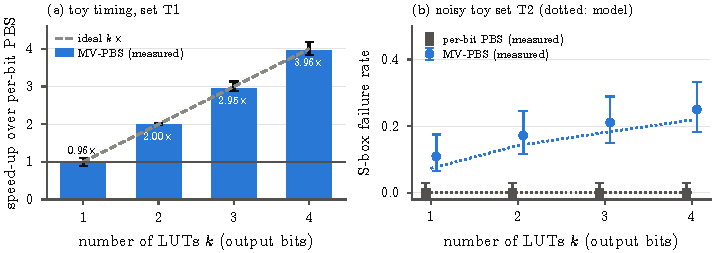
\includegraphics[width=\textwidth]{figs/fig_speedup_failure.pdf}
\caption{(a) Speed-up of \MVPBS{} over per-bit \PBSop{} versus the number of tables $k$ at T1,
bars with paired-bootstrap confidence intervals; dashed: $k\times$. (b) S-box failure rate
(any of the first $k$ bits wrong) at T2 with Wilson intervals; dotted: \Cref{thm:noise}.}
\label{fig:main}
\end{figure}

\noindent\textbf{Noise.} At T1, 0 of 384\evid{E16} evaluated output bits were wrong
(both methods). At T2 the per-bit \PBSop{} output has measured standard deviation
$2^{-8.54}$\evid{E14} (model $2^{-8.50}$\evid{E14}) and never fails (0/128, Wilson upper
end 0.029\evid{E12}), whereas the \MVPBS{} output for bit~0 has $2^{-6.74}$\evid{E13} (model
$2^{-6.84}$\evid{E13}) against a margin of $2^{-6}$\evid{E20}. The S-box failure rate grows with
the number of bits used, from 14/128 at $k=1$ to 32/128 at $k=4$, i.e.\ 0.25
[0.183, 0.332]\evid{E10}; \Cref{thm:noise} with an independence approximation predicts
0.219\evid{E18}. So one blind rotation for all four bits is safe only when the parameters are
chosen for the amplified noise.

\noindent\textbf{A remark on CMux trees.} Vertical packing~\cite{CGGI17} evaluates the whole
table with four CMux gates, but only from GGSW encryptions of the input bits. From a single
LWE ciphertext of the nibble this first requires extracting the bits and circuit-bootstrapping
each of them, which in our toy costs more than one \MVPBS{}; we therefore do not report it as a
competitor.
    % 7 Implementation and evaluation
% conclusion.tex (TEACHING EXAMPLE).
\section{Conclusion}\label{sec:conclusion}
Sharing one blind rotation among the four output bits of a 4-bit S-box, as proposed
in~\cite{CIM19}, gives a speed-up close to the number of bits in our toy, and the noise price
is exactly the factor $\|d_f\|^2\le p+2$ of \Cref{thm:noise}. Two lessons of the falsification
round carry over to real studies: speed-up claims must be checked at the edge of the claimed
range (the scaling saturates), and comparisons must start from the same input format.
\emph{Limitations:} insecure toy parameters, pure-Python timings, and a single S-box; nothing
here should be cited as a performance result.
     % 8 Conclusion

\ifanon\else
\subsubsection*{Acknowledgements.} Teaching example of the crypto-research-agents toolkit.
\fi

\bibliographystyle{splncs04}
\bibliography{../refs}  % single source: ../refs.bib (owner: lit-scout)

\appendix
% APPENDIX -- supplementary; reviewers are not obliged to read it, so nothing here
% may be load-bearing for the body's claims.
% appendix.tex (TEACHING EXAMPLE) -- nothing here is load-bearing.
\section{Reproducing the Case Study}\label{app:repro}
From the repository root:
{\small
\begin{verbatim}
cd case-study/toy-mvpbs
/usr/bin/python3 code/test_sbox_fhe.py
/usr/bin/python3 theory/check_mvpbs_noise.py
/usr/bin/python3 code/run_experiments.py
/usr/bin/python3 falsify/C3_linear_speedup/check_linear_speedup.py
/usr/bin/python3 code/make_figures.py
\end{verbatim}
}
The ledger \texttt{EVIDENCE.md} maps every number of this paper to a log under
\texttt{results/}; \texttt{CLAIMS.md} records which statements survived falsification.


\end{document}
